%

\section{Action Model for Synchronous Message Passing Protocol}
\label{sec:SMPactionmodel}

%
%

%
%
%
%
%
%
%

\subsection{Actions as posets of rank at most $1$} \label{subsec:actionAsPosets}

In the synchronous message passing protocol,
each agent sends its local private value to all the agents in the system.
%
When an agent crashes,
only the messages that have already been sent before the crash
are properly delivered to other agents; the rest are not.
In a synchronous distributed environment,
a correct agent can detect the exact set of crashed agents in the system:
An agent is dead (i.e., it has crashed), if no message is received from
the agent within a sufficiently long but finite period of time.
%
The protocol complex for the synchronous message passing protocol thus
forms an impure simplicial complex \cite{S1571:2001:HerlihyRajsbaumTuttle},
in which the vertexes corresponding to dead agents are missing in a facet.

%

%

%

%
%

%

%

%
%

%
%
%

In the impure protocol complex, 
each different facet arises from each different `pattern of failure' in
message delivery, where each specific pattern of failure
can be described by a set of orderings of the form $a < b$,
which means that the agent~$a$ has crashed and failed to send the message to the agent~$b$, 
a correct agent that did not crash.
This motivates us to define actions by relevant orderings over the set of agents
that satisfy the following properties.
\begin{itemize}
    \item An agent $a$ is dead after an action (i.e., the agent has crashed during the execution of the protocol)
          if and only if the corresponding poset of the action admits an ordering $a<b$ for some agent~$b$.
          %
    \item An agent $a$ is alive after an action
          if and only if the corresponding poset of the action does not admit
          an ordering $a<b$ for any agent~$b$.
          %
    \item If a poset contains an ordering $a<b$,
          the poset does not admit an ordering $c<a$ or $b<c$ for any agent~$c$.
          (This is because the ordering $a<b$ indicates that $a$ is a dead agent and
          $b$ is a correct agent but $c<a$ or $b<c$ implies otherwise.)
\end{itemize}

This ordering can be formalized as a poset (partially ordered set)
$(\Ag, \leq)$ of rank at most $1$.
A poset is of \keywd{rank}~$k$,
if the maximum number of elements contained
in a totally ordered subset of the poset is $k+1$. \cite{Book:2011:Stanley}
As usual, the strict ordering $a<b$ holds if and only if $a\leq b$ and $a\neq b$.

Let us define $\Lo(\leq) = \{ a \in \Ag \mid \exists b \in \Ag, a < b \}$
to denote the set of dead agents.
%
Notice that the reflexive ordering $a\leq a$ is not counted as a failure of message delivery.
We are not interested in the success or failure of self-delivery of message:
If successful, the agent~$a$ trivially receives its own local private value;
Otherwise, the agent~$a$ is dead and its received messages are lost.
In this respect, we indicate a poset by a set $S$ of strict orderings
and write $\Rcls{S}$ to denote the minimum poset containing $S$, i.e., the reflexive closure of $S$.
For example, $\Rcls{\{0<1, 2<3\}}$ defines a poset ordering $\leq$ over $\Ag$ such that
$a\leq b$ holds if and only if either $a=0$ and $b=1$,  $a=2$ and $b=3$, or $a=b$.
In particular, $\Rcls{\emptyset}$ is a discrete poset (of rank $0$) over $\Ag$,
in which any pair of distinct agents are incomparable.

\subsection{Constructing the action model $\ActSMP$} 
\label{subsec:constActModel}

%
%

Let us first consider the action model for the `inputless' case,
where the initial inputs to the agents are insignificant.
In this case, the actions for the synchronous message passing protocol is simply modeled 
by the posets over $\Ag$ of rank at most $1$.
%

\begin{definition} \label{def:smp_one}
    %
    %
    The \keywd{inputless action model} for synchronous message passing protocol is
    a partial epistemic frame 
    $\ActOneSMP = \langle T, \sim\rangle$ consisting of:
    \begin{itemize}
        \item The set of actions $
            T = \{
            t \mid t \text{ is a poset of rank at most $1$ over $\Ag$} \}$ and

        \item The family of indistinguishability relation, where $t_1 \sim_a t_2$ is defined 
        for each $a\in\Ag$ by: 
        \[
            t_1 \sim_a t_2 ~\text{ iff }~
            a \notin \Lo(t_1) \cup \Lo(t_2) \text{ and }
            \{ b \in \Ag \mid \SendFail{t_1}{b}{a} \} = \{ b \in \Ag \mid \SendFail{t_2}{b}{a} \}.
            \]
    \end{itemize}

    For each $t\in T$, we denote the set of live agents by 
    $\Alives{t} = \Ag \setminus \Lo(t)= \{ a \in \Ag \mid t \sim_a t \} $.    
\end{definition}


%
%
%
%

%
%
%

%
%
%
%
%
%
%
%

%
%
%
%
%
%
%
%
%

%

%

%
%
%
%
%
%

\begin{figure}[t]
    \begin{center}
        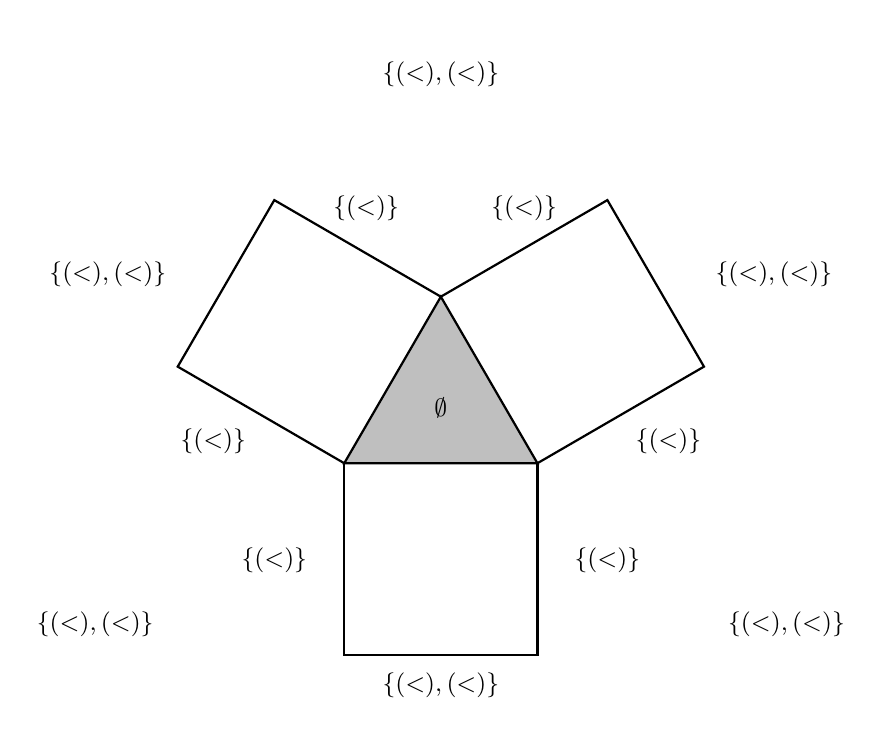
\begin{tikzpicture}[scale=1.41]
            \draw[fill=lightgray, thick](0,1)--(0.87,-0.5)--(-0.87,-0.5)--cycle;
            \draw(0,0)node{\small $\RefClosure{\emptyset}$};

            \draw[thick](0,1)--(1.5,1.87)--(2.37,0.37)--(0.87,-0.5);
            \draw(0.75,1.8)node{\small $\RefClosure{\{(\nodeW<\nodeB)\}}$};
            \draw(3,1.2)node{\small $\RefClosure{\{(\nodeW<\nodeB),(\nodeW<\nodeR)\}}$};
            \draw(2.05,-0.3)node{\small $\RefClosure{\{(\nodeW<\nodeR)\}}$};

            \draw[thick](0,1)--(-1.5,1.87)--(-2.37,0.37)--(-0.87,-0.5);
            \draw(-0.75,1.8)node{\small ~ $\RefClosure{\{(\nodeR<\nodeW)\}}$};
            \draw(-3,1.2)node{\small $\RefClosure{\{(\nodeR<\nodeB),(\nodeR<\nodeW)\}}$};
            \draw(-2.05,-0.3)node{\small $\RefClosure{\{(\nodeR<\nodeB)\}}$};


            \draw[thick](0.87,-0.5)--(0.87,-2.23)--(-0.87,-2.23)--(-0.87,-0.5);
            \draw(1.5,-1.37)node{\small $\RefClosure{\{(\nodeB<\nodeW)\}}$};
            \draw(-1.5,-1.37)node{\small $\RefClosure{\{(\nodeB<\nodeR)\}}$};
            \draw(0,-2.5)node{\small $\RefClosure{\{(\nodeB<\nodeW),(\nodeB<\nodeR)\}}$};

            \draw(0,1.0)node{\Large $\nodeB$};
            \draw(1.5,1.87)node{\Large $\nodeR$};
            \draw(2.37,0.37)node{\Large $\nodeB$};
            \draw(0.87,-0.5)node{\Large $\nodeR$};
            \draw(0.87,-2.23)node{\Large $\nodeW$};
            \draw(-0.87,-2.23)node{\Large $\nodeR$};
            \draw(-0.87,-0.5)node{\Large $\nodeW$};
            \draw(-2.37,0.37)node{\Large $\nodeB$};
            \draw(-1.5,1.87)node{\Large $\nodeW$};

            \draw(0,3.34)node{\Large $\nodeB$};
            \draw(0,3.0)node{\small $\RefClosure{\{(\nodeR<\nodeB),(\nodeW<\nodeB)\}}$};

            \draw(-2.9,-1.67)node{\Large $\nodeW$};
            \draw(-2.5,-1.95)node[anchor=east]{\small $\RefClosure{\{(\nodeB<\nodeW),(\nodeR<\nodeW)\}}$};

            \draw(2.9,-1.67)node{\Large $\nodeR$};
            \draw(2.5,-1.95)node[anchor=west]{\small $\RefClosure{\{(\nodeB<\nodeR),(\nodeW<\nodeR)\}}$};
        \end{tikzpicture}
    \end{center}
    \caption{The inputless action model $\ActOneSMP$ of the synchronous message passing protocol for $3$~agents, 
    with facets annotated by the corresponding posets over $\Ag$}
    \label{fig:3_protKripSmpOne}
\end{figure}



%
\begin{example}
    Figure~\ref{fig:3_protKripSmpOne} illustrates the complex of 
    the inputless action model $\ActOneSMP$ for $3$~agents. 
    The complex is impure, where the facet corresponding to an action $t$
    is of dimension $\abs{\AliveSet{t}}-1$. %
    When $t \sim_a^{\ActOneSMP} s$ holds, 
    the condition $a \notin \Lo(t) \cup \Lo(s)$ means that  
    the agent $a$ is alive for both actions $t$ and $s$; 
    The condition $\{ b \in \Ag \mid \SendFail{t}{b}{a} \} = \{ b \in \Ag \mid \SendFail{s}{b}{a} \}$
    means that $t$ and $s$ have the same set of agents that failed to send a message to~$a$
    and hence they know exactly the same set of delivered messages. 
    %
    For example, let 
    $t_1=\RefClosure{\{(\nodeB<\nodeR)\}}$, 
    $t_2=\RefClosure{\{(\nodeB<\nodeW), (\nodeB<\nodeR)\}}$, 
    $t_3=\RefClosure{\{(\nodeB<\nodeW)\}}$.  
    Then $t_1 \sim_{\nodeR}^{\ActOneSMP} t_2$ holds because, 
    in both $t_1$ and $t_2$, the agent~$\nodeR$ is alive 
    and has successfully received messages from 
    the agents other than $\nodeB$. 
    On the other hand, $t_1 \sim_{\nodeR}^{\ActOneSMP} t_3$ does not hold
    because the agent~$\nodeW$ in $t_3$ has received the messages from all
    the agents, but the same agent~$\nodeW$ in $t_1$ did not, from the
    agent $\nodeB$. 
\end{example}
%

From the inputless action model, 
we construct a full action model of the synchronous message passing protocol,
where the protocol accepts a class of sets of input values. 
Suppose $\Inpu$ is a simplicial model, whose facets specify the allowed combinations of input values. 
Then one might expect that an action in the full action model 
would be expressed by a pair $(X, t)$, where $X$ is a facet of $\Inpu$ 
and $t$ is an action of the inputless action,
but this does not give an appropriate model.
Consider the case, say, $t = \RefClosure{\{ b<a \}}$, 
$X \sim_{a}^{\Inpu} Y$, and $X \not\sim_{b}^{\Inpu} Y$. 
In this case, $(X, t)$ and $(Y, t)$ are different actions but the live
agent $a$ should not distinguish them because the action $t$ indicates
that the agent~$a$ has not received a message from the agent~$b$ and
therefore it cannot tell which is the original input, either $X$ or $Y$.
In other words, the two facets $X$ and $Y$ should be identified. 

For this identification of facets w.r.t.\ an action~$t$ of the inputless model,  
we introduce an equivalence class, written $\ActEquiv{t}{X}$,
and define an action in the full action model by a pair $(\ActEquiv{t}{X},t)$. 

%
%
%
%
%
%
%
%
%
%
%
%
%
%
%


%

\begin{definition}[action model of synchronous message passing]
    \label{def:SMP}    \label{def:sameLocalViewForAlives}
    Let $\Inpu = \SimpTuple{\Inpu}$ be an input simplicial model.
    For each facet $X, Y \in \Facet(\Inpu)$ and action $t \in \ActOneSMP$,
    we define an equivalence relation $\SameLocalViewForAlives{t}{X}{Y}$ by:
    \[
        \SameLocalViewForAlives{t}{X}{Y}
        \text{ iff }
        \forall a \in \Alives{t}.\:
        \forall b \in \Ag.\: (
            X \sim^{\Inpu}_b Y \vee \SendFail{t}{b}{a}
            ).
            %
            %
            %
            %
        \]
        We write $\ActEquiv{t}{X}$ to denote the equivalence class of $X$ w.r.t.\ 
        $\SameLocalViewForAlivesOp{t}$. 
    
    We define
    the action model $\ActSMP=\anglpair{T^{\ActSMP}, \sim^{\ActSMP}, \PreOp^{\ActSMP}}$ of
    the synchronous message passing protocol as a triple consisting of:
    \begin{itemize}
        \item The set of actions 
        $T^{\ActSMP} = \{ (\ActEquiv{t}{X}, t) \mid X \in \Facet(\Inpu),~ t \in \ActOneSMP \}$;
        \item The family of indistinguishability relations defined by 
        \[
            (\ActEquiv{t}{X}, t) \sim^{\ActSMP}_a (\ActEquiv{s}{Y}, s)
              ~\text{ iff }~
              t \sim^{\ActOneSMP}_a s
              \text{ and }
              \forall b \in \Ag.\: (X \sim^{\Inpu}_b Y \vee \SendFail{t}{b}{a});
              %
              %
          \]
        %
        \item The precondition defined by
        $
        \PreOp^{\ActSMP} \bigl((\ActEquiv{t}{X}, t)\bigr)
                  = \bigvee \{
                  \bigwedge \labSM^{\Inpu}(Y) \mid Y \in \ActEquiv{t}{X}
                  \}
              $. %
    \end{itemize}
\end{definition}

%
%
%
%
%
%
%
%
%
%
%
%
%
%
%
%
%
%
%
%
%
%
%


In words, $\SameLocalViewForAlives{t}{X}{Y}$ indicates that,
for every agent $a$ that is alive in the action $t$, 
$X$ and $Y$ should have the same input for the agent~$b$, if 
$\NotSendFail{t}{b}{a}$, i.e., the message from~$b$ is successfully 
received by $a$. (Otherwise, the agent~$a$ should be aware that 
$X$ and $Y$ are different facets.)
The relation $\SameLocalViewForAlivesOp{t}$ is an equivalence relation, 
as we will show below. 
%
%
The relation $\sim^{\ActSMP}_a$ defines a PER, where 
$(\ActEquiv{t}{X}, t) \sim^{\ActSMP}_a (\ActEquiv{s}{Y}, s)$
indicates that the agent~$a$ is alive
and every agent~$b$ that successfully sends a message to~$a$
(i.e., $\NotSendFail{t}{b}{a}$) has the same input value that has been assigned 
in both $X$ and $Y$.  
%
The precondition $\PreOp^{\ActSMP} \bigl((\ActEquiv{t}{X}, t)\bigr)$ is 
intended to mean that, for an action $(\ActEquiv{t}{X}, t)\in T^{\ActSMP}$, 
every atomic proposition in $\labSM^{\Inpu}(Y)$ is true 
for some $Y \in \ActEquiv{t}{X}$.  


%
%
%
%
%
%
%

%
%
%
%
%
%
%
%

%
%
%


\begin{proposition}
    \label{prop:actSimWellDefined}
    Let $\Inpu$ be an input simplicial model. 
    For every $t\in \ActOneSMP$, $\SameLocalViewForAlivesOp{t}$ is an equivalence relation. 
    Furthermore, the relation $\sim^{\ActSMP}_a$ is a PER and is well-defined. 
    That is, $\sim^{\ActSMP}_a$ is a symmetric transitive relation and is not affected by
    the choice of facet $X$ %
    in $(\ActEquiv{t}{X},t)$.
\end{proposition}

%
%
%
%
%

\begin{proof}
    Obviously, $\SameLocalViewForAlivesOp{t}$ is a reflexive symmetric relation. 
    For transitivity, assume $\SameLocalViewForAlives{t}{X}{Y}$ and $\SameLocalViewForAlives{t}{Y}{Z}$.
    Suppose $X \not\sim^{\Inpu}_b Z$. By the transitivity of $\sim^{\Inpu}_b$, 
    we have $X \not\sim^{\Inpu}_b Y$ or $Y \not\sim^{\Inpu}_b Z$. 
    In both cases, we have $\SendFail{t}{b}{a}$ for all $a\in\Ag$. 
    Hence $\SameLocalViewForAlives{t}{X}{Z}$. 

    To show that $\sim^{\ActSMP}_a$ is symmetric, suppose 
    $(\ActEquiv{t}{X}, t) \sim^{\ActSMP}_a (\ActEquiv{s}{Y}, s)$. 
    By the definition, $t \sim^{\ActOneSMP}_a s$ and 
    $\forall b \in \Ag.~(X \sim^{\Inpu}_b Y \vee \SendFail{t}{b}{a})$.
    Since $t \sim^{\ActOneSMP}_a s$ implies 
    $\{ b \in \Ag \mid \SendFail{t}{b}{a} \} = \{ b \in \Ag \mid \SendFail{s}{b}{a} \}$, 
    by the symmetry of $\sim^{\ActOneSMP}_a$ and $\sim^{\Inpu}_b$, 
    we have $(\ActEquiv{s}{Y}, s) \sim^{\ActSMP}_a (\ActEquiv{t}{X}, t)$. 
    The transitivity of $\sim^{\ActSMP}_a$ follows similarly from
    the transitivity of $\sim^{\ActOneSMP}_a$ and $\sim^{\Inpu}_b$. 

    %
    %
    %

    %
    %
    %
    %
    %
    %
    %
    %


    For the well-definedness of $\sim^{\ActSMP}_a$, 
    suppose $(\ActEquiv{t}{X}, t) \sim^{\ActSMP}_a (\ActEquiv{s}{Y}, s)$, 
    $\ActEquiv{t}{X}=\ActEquiv{t}{X'}$, and 
    $\ActEquiv{s}{Y}=\ActEquiv{s}{Y'}$. We show
    $(\ActEquiv{t}{X'}, t) \sim^{\ActSMP}_a (\ActEquiv{s}{Y'}, s)$. 
    Since $\sim^{\ActOneSMP}_a$ is a PER, it suffices to show 
    that $\forall b \in \Ag.~(X' \sim^{\Inpu}_b Y' \vee \SendFail{t}{b}{a})$.
    Assume otherwise, i.e., $X' \not\sim^{\Inpu}_b Y'$ and $\NotSendFail{t}{b}{a}$
    holds for some $b\in\Ag$. Then, from
    $(\ActEquiv{t}{X}, t) \sim^{\ActSMP}_a (\ActEquiv{s}{Y}, s)$, 
    we have $a \in \Alives{t}$ and $a \in \Alives{s}$
    and also entail $X \sim^{\Inpu}_b Y$ from $\NotSendFail{t}{b}{a}$. 
    Since $\SameLocalViewForAlives{t}{X}{X'}$, we have $X \sim^{\Inpu}_b X'$.
    Similarly, $Y \sim^{\Inpu}_b Y'$. By the transitivity of 
    $\sim^{\Inpu}_b$, we obtain $X' \sim^{\Inpu}_b Y'$, a contradiction. 
    %
    %
    %
    %
    %
    %
    %
    %
    %
    %
    %
    %
    %
\end{proof}

%
%
%
%
%
%
%
%
%
%
%
%
%

%
%
%

%
%

%
%
%
%
%
%
%
%
%
%
%

%
%
%

%
%
%

%
%
%
%
%
%
%
%
%
%
%
%
%

%
%
%
%
%
%
%
%
%
%
%
%
%
%
%


%
%
%
%


%
%
%
%
%
%
%
%
%


    \begin{figure}[t]
        %
        %
        %
        %
        %

        %

        %
        %
        %
        %
        %
        %
        %
        %
        %
        %
        %
        %
        \centering
        %
            %
                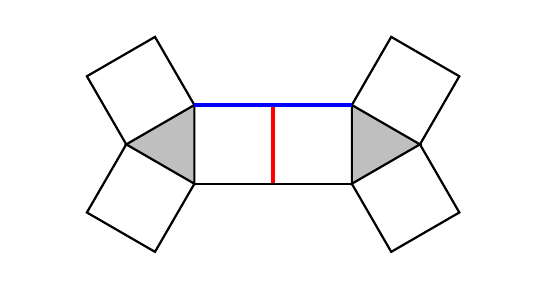
\begin{tikzpicture}[scale=0.5]
                    \draw[fill=lightgray, thick](2,1)--(2,-1)--(3.73,0)--cycle;

                    \draw[fill=lightgray, thick](-2,1)--(-2,-1)--(-3.73,0)--cycle;

                    \draw[thick](2,1)--(-2,1);

                    \draw[thick](2,-1)--(-2,-1);
                    \draw[thick](0,1)--(0,-1);

                    \draw[thick](2,1)--(3,2.73)--(4.73,1.73)--(3.73,0);
                    \draw[thick](2,-1)--(3,-2.73)--(4.73,-1.73)--(3.73,0);

                    \draw[thick](-2,1)--(-3,2.73)--(-4.73,1.73)--(-3.73,0);
                    \draw[thick](-2,-1)--(-3,-2.73)--(-4.73,-1.73)--(-3.73,0);

                    \draw[very thick, red] (0, 1) -- (0, -1);
                    \draw[very thick, blue] (-2, 1) -- (2, 1);
                    \draw[thick] (-2, -1) -- (2, -1);

                    %

                    \draw (0, 2.73) node {\Large $\nodeR$};
                    \draw (0, -2.73) node {\Large $\nodeW$};
                    \draw (-6.0, 0) node {\Large $\nodeB$};
                    \draw (6.0, 0) node {\Large $\nodeB$};

                    \draw(0,1)node{\Large $\nodeW$};
                    \draw(0,-1)node{\Large $\nodeR$};

                    \draw(2,1)node{\Large $\nodeR$};
                    \draw(2,-1)node{\Large $\nodeW$};
                    \draw(3.73,0)node{\Large $\nodeB$};
                    \draw(3,2.73)node{\Large $\nodeB$};
                    \draw(4.73,1.73)node{\Large $\nodeR$};
                    \draw(3,-2.73)node{\Large $\nodeB$};
                    \draw(4.73,-1.73)node{\Large $\nodeW$};

                    \draw(-2,1)node{\Large $\nodeR$};
                    \draw(-2,-1)node{\Large $\nodeW$};
                    \draw(-3.73,0)node{\Large $\nodeB$};
                    \draw(-3,2.73)node{\Large $\nodeB$};
                    \draw(-4.73,1.73)node{\Large $\nodeR$};
                    \draw(-3,-2.73)node{\Large $\nodeB$};
                    \draw(-4.73,-1.73)node{\Large $\nodeW$};
                \end{tikzpicture}
            %
        %

        \caption{An action model $\ActSMP$ for $3$ agents, 
                generated from an input model consisting of two facets}
        \label{fig:3_smp_two_simplicial}
    \end{figure}

\begin{example} \label{eg:smpTwo}
    Let us consider an input simplicial model $\cplI$ for $3$~agents,  
    consisting of  two facets $X = \{ (\nodeW, 0), (\nodeR, 0), (\nodeB, 0) \}$ and 
    $Y = \{ (\nodeW, 0), (\nodeR, 0), (\nodeB, 1) \}$.
    %
    %
    Then we obtain the action model $\ActSMP$ as depicted in Figure~\ref{fig:3_smp_two_simplicial}. 
    We obtain this complex by first making copies of the complex of the inputless action model,
    for each facet $X$ and $Y$, and pasting them appropriately. 
    For example, the action represented by the poset $t=\RefClosure{\{\nodeB<\nodeW, \nodeB<\nodeR\}}$ 
    generates two copies $(\ActEquiv{t}{X}, t)$ and $(\ActEquiv{t}{Y}, t)$, but 
    these are identified (as depicted by the $1$-dimensional simplex marked by the red line in the figure)
    because $\ActEquiv{t}{X} = \ActEquiv{t}{Y} = \{X, Y\}$.
    Similarly, the topmost node $\nodeR$ and the bottom node~$\nodeW$ in the figure
    identify the corresponding $0$-dimensional simplexes in the copies generated from $X$ and $Y$. 

    Consider another action $s=\RefClosure{\{\nodeB<\nodeW, \nodeB<\nodeR\}}$.
    This generates two copies $(\ActEquiv{s}{X}, s)$ and $(\ActEquiv{s}{Y}, s)$, 
    which are depicted in the figure by the two $1$-dimensional simplexes marked by the blue lines.
    These simplexes are connected via a common vertex $\nodeW$. That is, 
    $(\ActEquiv{s}{X}, s) \sim_{\nodeW}^{\ActSMP} (\ActEquiv{s}{Y}, s)$ holds,
    since $X \sim_{\nodeR}^{\Inpu} Y$ and $\nodeR$ is the only agent $b$
    that satisfies $\NotSendFail{s}{b}{\nodeW}$.
    The two simplexes are not identified nevertheless, since 
    $(\ActEquiv{s}{X}, s) \not\sim_{\nodeR}^{\ActSMP} (\ActEquiv{s}{Y}, s)$ 
    follows from $X \not\sim_{\nodeR}^{\Inpu} Y$ and 
    $\NotSendFail{s}{\nodeR}{\nodeW}$.

    %
    %

    %

    %
    %
    %
    %
    
    %
    %
    %
    %
    %
    %
    %
    %
    %
    %
    %

    %
    %
    %
\end{example}
